% Generated by figures/make_figures.py from numbers.tex; do not edit.
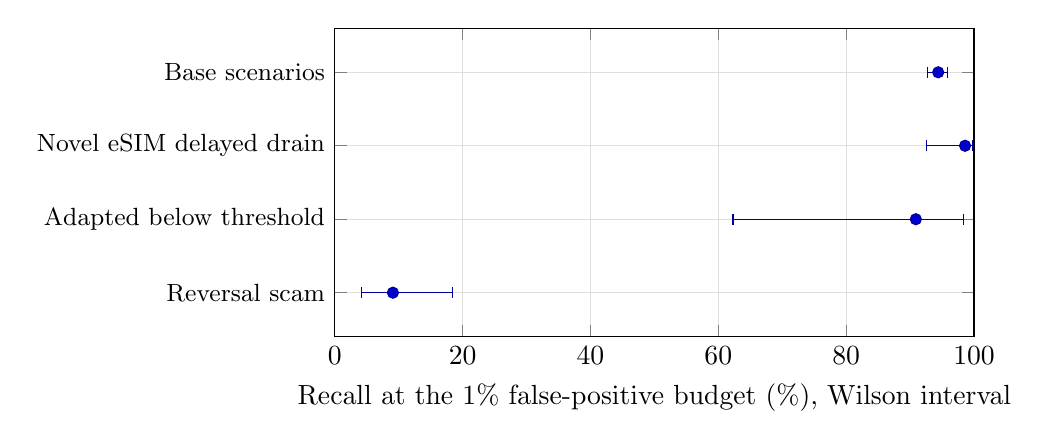
\begin{tikzpicture}
  \begin{axis}[
      width=0.8\linewidth, height=5.5cm,
      xmin=0, xmax=100, xlabel={Recall at the 1\% false-positive budget (\%), Wilson interval},
      symbolic y coords={{Base scenarios},{Novel eSIM delayed drain},{Adapted below threshold},{Reversal scam}},
      ytick=data, y dir=reverse, yticklabel style={font=\small}, enlarge y limits=0.2,
      grid=major, grid style={gray!25},
    ]
    \addplot+[only marks, mark=*, blue!60!black,
      error bars/.cd, x dir=both, x explicit] coordinates {
      (94.4,{Base scenarios}) -= (1.7,0) += (1.4,0)
      (98.6,{Novel eSIM delayed drain}) -= (6.0,0) += (1.2,0)
      (90.9,{Adapted below threshold}) -= (28.6,0) += (7.5,0)
      (9.1,{Reversal scam}) -= (4.9,0) += (9.3,0)
    };
  \end{axis}
\end{tikzpicture}
